\section*{Résumé}
Les cellules solaires photovoltaïques sont généralement modélisées avec un circuit électrique comprenant un certain nombre de paramètres.

\section*{Abstract}
Solar PV cells are generally represented by a lumped-element model with a set number of components which are represented by their parameters. These parameters are not readily available in manufacturer data-sheets despite being crucial to the accuracy of the model. A possible approach is to estimate these parameters using the Current-Voltage characteristic of a cell using numerical or analytic techniques. Metaheuristics such as Differential Evolution take the approach of an optimization with the objective function to be minimized being the error with experimental Current-Voltage data. This work is a comparative analysis between different combinations of methods such as Differential Evolution and Particle Swarm Optimization applied to the single and double diode models for various solar cell technologies. PSO is used to initially cover the entire multidimensional search space in order to find a region with global minimum, which is subsequently given to the DE algorithm in order to locate the solution with the best fitness within this region. A small tool implementing these methods has been developed using the Python programming language.

\section*{Nomenclature}
\noindent\textbf{GHG} \hfill Green House Gas \hfill Gaz à effet de serre\\
\textbf{DE} \hfill Differential Evolution \hfill \phantom{}\\
\textbf{$E_g$} \hfill Bandgap\\
\textbf{EQE} \hfill External Quantum Efficiency\\

\newpage
\tableofcontents
\newpage

\chapter*{Introduction Générale}
\label{sec:intro}
\addcontentsline{toc}{section}{\nameref{sec:intro}}
%inexhaustible en principe
L’épuisement des énergies fossiles et leur nature non-durable a conduit à la croissance rapide des énergies renouvelables comme sources alternatives d'énergie. L’énergie solaire est l’une de ces sources renouvelables les plus répandues et a prouvé son utilité dans plusieurs domaines d'applications grâce à sa nature quasiment inexhaustible en principe. Les technologies photovoltaïques en particulier ont fait l'objet intense d'étude de la part de la communauté scientifique depuis la première cellule en silicone cristallin à 6\% de Chapin et al. \cite{Chapin1954} en 1954. Ceci a entraîné une croissance considérable de l'industrie photovoltaïques. En fait, la capacité de production en PV a dépassé les 150GW \cite{iea2020} en 2019 (figure \ref{fig:ieapv}), ce qui correspond une croissance d'environ 100GW depuis 2014. Les décennies de recherche depuis la cellule de Chapin et al. visent généralement l'amélioration des cellules solaires \textit{(i)} en explorant les différentes architectures possibles des cellules, \textit{(ii)} en développant des matériaux qui permettent d'augmenter l'efficacité de conversion de l'énergie solaire incidente ou \textit{(iii)} en réduisant le coût du processus de production. La première génération des technologies PV se basait sur des wafer de Silicone comme matériau actif de conversion. La deuxième génération remplace le silicone avec des semi-conducteurs à couches minces, qui, parmi d'autres avantages, réduit considérablement les besoins en matières premières (silicone). Les troisièmes et futures générations comprennent les cellules organiques, Perovskite et les Quantum Dots et présentent des pistes d'investigations pour réduire davantage les coûts de production et augmenter l'efficacité de conversion.\\
Le principe de fonctionnement des cellules photovoltaïques a été discuté en profondeur dans la littérature \cite{Fraas2010,  Sze2006, Wenham2013}.
Les photons à énergie supérieure au bandgap du matériau semi-conducteur sont absorbé en transférant leur énergie aux électrons dans la bande de valence, ce qui leur permet de passer vers la bande de conduction en laissant un "trou" derrière. Le rôle du champ électrique présent dans la zone de déplétion des jonctions P-N est de séparer ces paires électron-trou et leur permettre de circuler à travers une charge extérieure. Toutefois, il y aurait toujours un plafond sur ce mécanisme de conversion "lumière $\rightarrow$ électricité" pour les cellules mono-jonction selon la limite Schockley-Queisser (SQ) \cite{Shockley1961}. Le modèle SQ postule que tous les photons à énergie supérieure au gap $E_g$ sont absorbés et que la totalité des recombinaisons qui surviennent sont strictement l'inverse du processus d'absorption, c'est-à-dire des recombinaisons radiatives qui re-emettent des photons.\\
Cependant, la performance d'une cellule réelle sera toujours inférieure à la limite SQ (figure \ref{fig:natsq}). Les mécanismes idéaux postulés par le formalisme de SQ sont affectés dans la pratique par plusieurs phénomènes imprévu qui parviennent des propriétés des matériaux utilisés. A titre d'exemple, la présence des défauts dans un semi-conducteur entraîne des recombinaisons non-radiatives où l'énergie des électrons est libérée en phonons dans la structure cristalline et non pas en lumière, ce qui génère de la chaleur dans le semi-conducteur. Les difficultés qui limitent les technologies PV nécessitent une meilleure compréhension des phénomènes physiques complexes impliqués, et l'étude de la performance des cellules par rapport au modèle SQ donne des indices sur la nature des gains en performance qu'une technologie particulière à le potentiel de réaliser.\\
La modélisation des cellules solaires est essentielle pour la conception, l'analyse et l'estimation de la performance des cellules solaires. Elle permet d'effectuer l'analyse des propriétés électriques pendant leur phase de développement, l'émulation des systèmes PV pour la prédiction des rendements énergétiques \cite{Ram2018}, le contrôle de qualité des cellules en phase de production %\cite{} 
et l'étude des effets de dégradation pendant la phase d'opération \cite{Kennerud1969, Jamil2017}. Bien qu'il y a des méthodes de simulations des phénomènes physiques dans la cellule comme celles qui reposent sur la dynamique moléculaire, la théorie fonctionnelle de la densité ou tout simplement des méthodes numériques appliquées aux équations des semi-conducteurs (équation de Poisson et équations de continuité) etc. Dans ce travail nous nous intéressons à l'approche des circuits équivalents à éléments localisés qui modélisent le comportement I-V de la cellule.\\
La modélisation d'éléments localisés permet de décrire le comportement des phénomènes physiques dispersés spatialement avec un ensemble d'éléments localisés dont chacun représente un phénomène physique particulier. L'analogie électrique dans les problèmes de transferts de chaleur est un exemple de cette méthode où une résistance localisée dans le modèle pourrait représenter la résistance thermique spatialement distribuée selon l'épaisseur de la paroi concernée. Dans le cas des cellules PV, chaque élément du circuit équivalent représente aussi un phénomène physique spécifique dans la cellule (e.g. une résistance en série modélise les pertes ohmiques causées par la résistance intrinsèque au semi-conducteur utilisé). La caractéristique I-V dépends des paramètres associés aux éléments localisés du circuit. Il s'agirait donc d'essayer de minimiser l'erreur entre la courbe caractéristique du modèle et celle de la cellule réelle en jouant sur les valeurs des paramètres. 
Pour ce faire, il existe deux approches principales. La première est l'approche analytique. Elle consiste à utiliser les données sur les points clés de la courbe caractéristique (tension circuit ouvert, courant court circuit, la pente de la courbe en ces points, ou encore le point de puissance maximale etc) et à effectuer certaines simplifications pour concevoir des formules approximatives, mais rapide à calculer. Toutefois, les simplifications effectuées peuvent conduire à des résultats imprécis ou non physiques (e.g. résistance négative). Le fait que cette approche utilise les données des quelques points seulement la rend vulnérable au bruit de mesures. La deuxième approche est l'extraction numérique. On se retrouve avec un problème d'optimisation, dont la fonction objective à extrémiser (minimiser) est l'erreur entre le modèle et la courbe expérimentale de la cellule réelle. L'algorithme utilisé pour l'optimisation en soi pourrait être déterministe comme dans le cas des méthodes de Newton-Raphson, Levenberg–Marquardt etc ou des algorithmes stochastiques/métaheuristique tel que les techniques évolutionnaires. Ces dernières comprennent l'algorithme génétique (GA), Particle Swarm Optimization (PSO), Recuit Simulé (SA) etc. Les méthodes déterministes imposent généralement des critères de convexité, différentiabilité (et par conséquent continuité) de la fonction objective. Bien qu'elles soient efficaces en terme d'optimisation locale avec des données de gradient, elles sont très susceptibles à se piéger dans des extremums locaux, ce qui limite leurs capabilités d'optimisation globale. Par contre les métaheuristiques n'ont pas d'exigences sur la fonction objective, et le choix des conditions initiales appropriées les rends plus robuste envers les pièges d'extremums locaux.\\
Dans ce travail..
\begin{figure}
  \begin{center}
    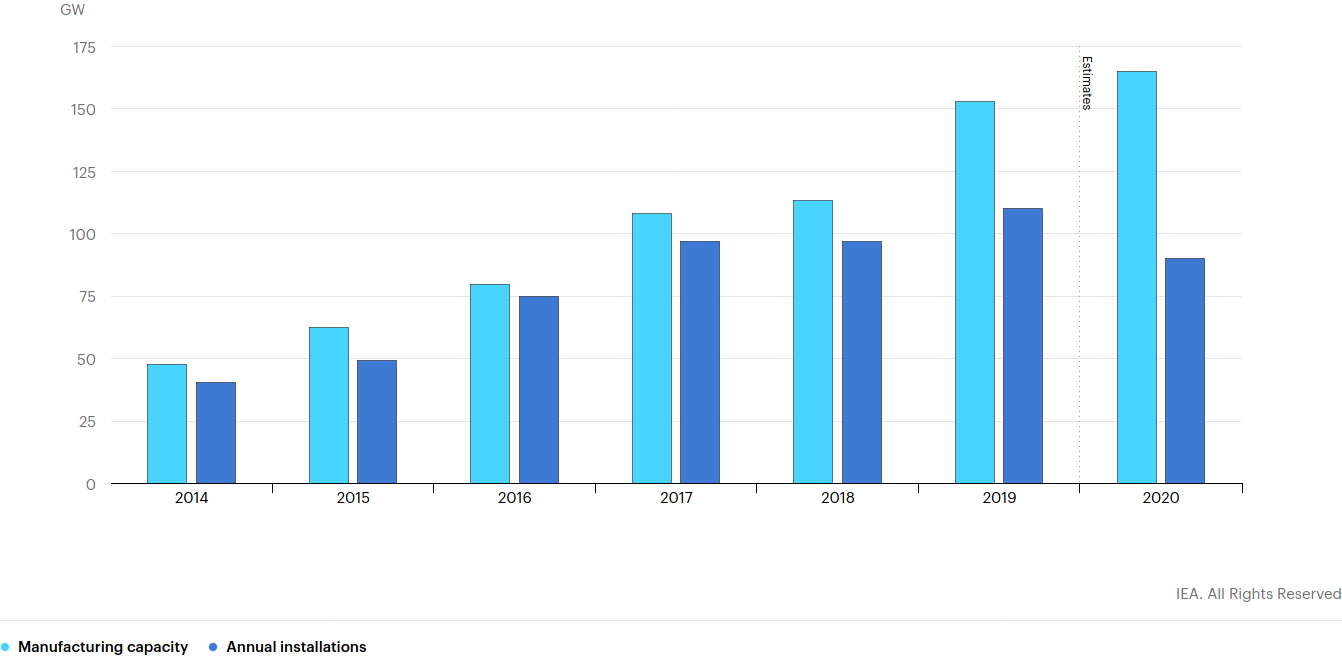
\includegraphics[width=\textwidth]{resources/ieapv.png}
    \caption{Fabrication et demande des modules solaires photovoltaïques, 2014-2020. Source: IEA analysis based on Paula Mints (2020), The Solar Flare, SVP Market Research, San Francisco, CA \cite{iea2020}}
    \label{fig:ieapv}
  \end{center}
\end{figure}
\begin{figure}
  \begin{center}
    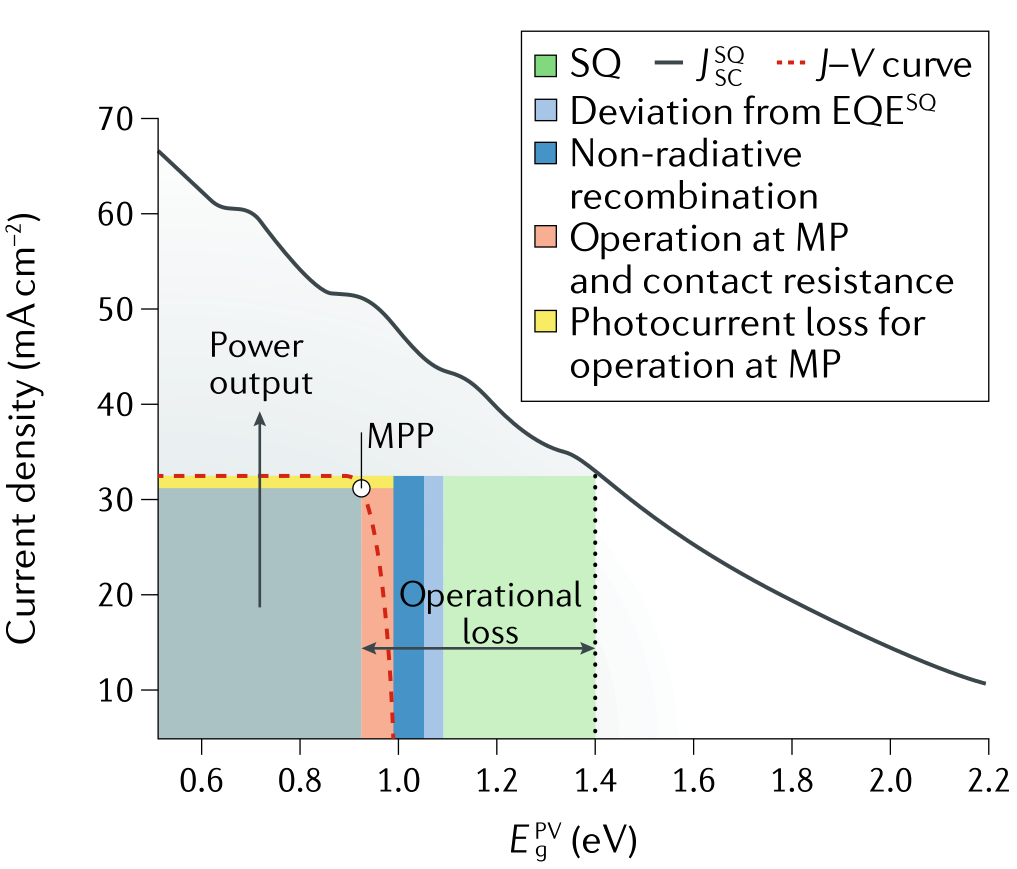
\includegraphics[width=0.5\textwidth]{resources/natsq.png}
    \caption{Différence entre le formalisme de SQ et une cellule réelle. Le photo-courant maximal CC à la limite de Schockley-Queisser est tracé en fonction du gap ($E_{g}^{PV}$). La ligne pointillée en rouge indique la caractéristique J-V de la cellule \cite{nayak2019}}
    \label{fig:natsq}
  \end{center}
\end{figure}
